\documentclass[10pt,xcolor={dvipsnames},aspectratio=169]{beamer}
%\documentclass[10pt,xcolor={dvipsnames},handout]{beamer}

%% option passed to the theme
\usetheme[
  color={default}, % feather, navy, dark, UHECE, SPWLA (SPWLA is default)
%  progressstyle=fixedCircCnt,   % fixedCircCnt, movingCircCnt (moving is deault)
]{SPWLA}

%-------------------------------------------------------
% Configure citations
%-------------------------------------------------------

% add two files
\addbibresource{bib/ref_nn.bib}
\addbibresource{bib/ref_superrs.bib}

%-------------------------------------------------------
% INDIVIDUAL COLORS
%-------------------------------------------------------

% The elements of the template can be changed individually. Note that you may
% need to use different colors in beamer / handout mode, when using the following
% methods:

% Change the bar colors:
% \setbeamercolor{SPWLA}{fg=NavyBlue!20,bg=NavyBlue}

% Change the color of the structural elements:
% \setbeamercolor{structure}{fg=NavyBlue}

% Change the frame title text color:
% \setbeamercolor{frametitle}{fg=black!5,bg=NavyBlue}

% Change the normal text colors:
% \setbeamercolor{normal text}{fg=black!75,bg=gray!5}

% Change the block title colors
% \setbeamercolor{block title}{use=Feather, bg=Feather.bg!20!black, fg=Feather.fg} 

%-------------------------------------------------------
% IMAGE FILES
%-------------------------------------------------------

% Change the logo in the upper right elipses:
%\renewcommand{\logofile}{example-grid-164x100pt} 
%% This is an image that comes with the LaTeX installation
% Adjust scale of the logo w.r.t. the circle; default is 0.875
% \renewcommand{\logoscale}{0.55}

% optional, add the second logo to the title page.
\setLogo{SPWLAGraphics/uhlogo}

% optional, add the background image to the final page.
\setFinalImage{SPWLAGraphics/cullen}

%-------------------------------------------------------
% INCLUDE PACKAGES
%-------------------------------------------------------

\usepackage[american]{babel}
% \usepackage{helvet}

%% Load different font packages to use different fonts
%% e.g. using Linux Libertine, Linux Biolinum and Inconsolata
% \usepackage{libertine}
% \usepackage{zi4}

%% e.g. using Carlito and Caladea
\usepackage{carlito}
\usepackage{caladea}
\usepackage{zi4}

%% e.g. using Venturis ADF Serif and Sans
% \usepackage{venturis}

%-------------------------------------------------------
% INFORMATION IN THE TITLE PAGE
%-------------------------------------------------------

% [] is optional - is placed on the bottom of the sidebar on every slide
\title[SPWLA Theme]
{ % is placed on the title page
  \textbf{The SPWLA Beamer Theme}
}

% subtitle is optional.
%\subtitle[v. 1.1.0]
%{
%\textbf{v. 1.1.0}
%}

% author is required. Use \texorpdfstring to configure hyperref correctly.
\author[Author 1]
{Author 1\texorpdfstring{\footnotemark[1]}{},
Author 2\texorpdfstring{\footnotemark[2]}{},
\texorpdfstring{$\cdots$}{...}
\texorpdfstring{ \\
  {\ttfamily author1@gmail.com}
}{}}

% institute is required. Will be shown in the title.
\institute[]
{%
  \footnotemark[1]Affiliation 1\\
  \footnotemark[2]Affiliation 2
}

% Meeting name is optional. If not given, will use default name.
\meeting{
  2022 spring topical conference\\petrophysical machine learning
}

% date is required. will be shown on each page.
\date{\today} % Could be configured as \today or a manually specified date: \formatdate{day}{month}{year}

%-------------------------------------------------------
% THE BODY OF THE PRESENTATION
%-------------------------------------------------------

\begin{document}

%-------------------------------------------------------
% THE TITLEPAGE
%-------------------------------------------------------

\titleframe

\begin{frame}{Content}{}
\tableofcontents
\end{frame}

%-------------------------------------------------------
\section{Introduction}
%-------------------------------------------------------
\subsection{License}
\begin{frame}{Introduction}{License}
%-------------------------------------------------------

  \begin{itemize}
    \item<1-> This template is modified from \chref{https://www.overleaf.com/latex/templates/beamer-presentation-template-feather-theme/jcbpcdxqbxbf}{Feather theme}. The GPLv3 is copied from the original template to this one.
    \item<2-> The \texttt{beamer} (default) style of this template is modified according to the standard of SPWLA 2022 conference. The original feather style is moved to \texttt{handout} mode.
    \item<3-> The rest of the theme is provided under the GNU General Public License v. 3 (GPLv3) \chref{http://www.gnu.org/licenses/}{http://www.gnu.org/licenses/}. This means that you can redistribute it and/or modify it under the same license. 
  \end{itemize}
\end{frame}

%-------------------------------------------------------
\section{Installation}
%-------------------------------------------------------
\subsection{Source files}
\begin{frame}{Installation}{Source files}
%-------------------------------------------------------

\begin{block}{}
The theme contains 4 source files:
  \begin{itemize}
    \item {\tt beamercolorthemeSPWLA.sty}
    \item {\tt beamerouterthemeSPWLA.sty}
    \item {\tt beamerinnerthemeSPWLA.sty}
    \item {\tt beamerthemeSPWLA.sty}
  \end{itemize}
\end{block}
\end{frame}

%-------------------------------------------------------
\subsection{Local and Global installation}
\begin{frame}{Installation}{Local and Global installation}
%-------------------------------------------------------
  The theme can be installed for \textbf{local} or \textbf{global} use.
  \pause
  \begin{block}{Local Installation}
  \begin{itemize}    
    \item Local installation is the simplest way of installing the theme. 
    \item You need to placing the 4 source files in the same folder as your presentation. When you download the theme, the 4 theme files are located in the {\tt local} folder.
  \end{itemize}
  \end{block}

  \begin{block}{Global Installation}
  \begin{itemize}
     \item If you wish to make the theme globally available, you must put the files in your local latex directory tree. The location of the root of the local directory tree depends on your operating system and the latex distribution. 
     \item Detailed steps on how to proceed installation under various operating systems can be found at Beamer documentation.
  \end{itemize}
  \end{block}
\end{frame}
     

%-------------------------------------------------------
\subsection{Required Packages}
\begin{frame}{Installation}{Required Packages}
%-------------------------------------------------------

  For using the basic \texttt{SPWLA} Theme you will need the Bemaer class installed and the following 5 packages
  \begin{itemize}
    \item \texttt{TikZ}\footnote{TikZ is a package for creating beautiful graphics. Have a look at these \chref{http://www.texample.net/tikz/examples/}{online examples} or the \chref{http://tug.ctan.org/tex-archive/graphics/pgf/base/doc/generic/pgf/pgfmanual.pdf}{pgf user manual}.}
    \item \texttt{tcolorbox}\footnote{tcolorbox is a package for creating customized blocks. To learn details, see \chref{http://tug.ctan.org/tex-archive/macros/latex/contrib/tcolorbox/tcolorbox.pdf}{tcolorbox user manual}.}
    \item \texttt{datetime}\footnote{datetime is required for formatting the date.}
    \item \texttt{textcase}\footnote{textcase is required for providing uppercase filter.}
    \item \texttt{calc}\footnote{calc is required for calculating the space and length of the object in this templates.}
  \end{itemize}
  Due to the fact that the packages are very common they should be included in your latex distribution in the first place.
\end{frame}

\begin{frame}{Installation}{Required Packages}
More required packages for advanced utilities:
\begin{itemize}
  \item \textbf{Citation}: \texttt{csquotes}, \texttt{biblatex}\footnote{biblatex is the best way to show citations in beamer, however, it may cause compatibility problems.}, \texttt{cleveref}\footnote{cleveref is the best way to create auto references, however, it may cause compatibility problems.}
  \item \textbf{Font}: \texttt{fontenc}
  \item \textbf{Environment}: \texttt{float}, \texttt{algorithm}, \texttt{algorithmic}, \texttt{subfigure}
  \item \textbf{Others}: \texttt{tabularx}, \texttt{array}, \texttt{siunitx}, \texttt{colortbl}
\end{itemize}
\end{frame}

%-------------------------------------------------------
\section{User Interface}
\subsection{Loading Beamer}
\begin{frame}{User Interface}{Loading Beamer with different mode}
%-------------------------------------------------------
  \vspace{-0.5em}
  \begin{block}{The Beamer Mode}
    \small
    The SPWLA can be loaded in two different \texttt{beamer} modes. The default mode is\\
    {\tt \textbackslash documentclass[<options>]\{beamer\}}\\
    Here \texttt{<options>} can be either \texttt{beamer} (by default) or \texttt{handout}.
  \end{block}
  \begin{block}{The Page Size}
    \small
    The size of the page can be configured in class options\\
    {\tt \textbackslash documentclass[aspectratio=169]\{beamer\}}\\
    {\tt \textbackslash documentclass[aspectratio=43]\{beamer\}}\\
    According to the standard of SPWLA, we recommend users to use 16:9 in \texttt{beamer} (presentation) mode.
  \end{block}
\end{frame}


%-------------------------------------------------------
\subsection{Loading the Theme and Theme Options}
\begin{frame}{User Interface}{Loading the Theme and Theme Options}
%-------------------------------------------------------
  \vspace{-0.5em}
  \begin{block}{The Presentation Theme}
    \small
    The SPWLA Theme can be loaded in a familiar way. In the reamble of your {\tt tex} file you must type\\
    {\tt \textbackslash usetheme[<options>]\{SPWLA\}}\\
    The presentation theme loads the inner, outer and color Feather theme files and passes the {\tt <options>} on to these files.
  \end{block}
  \begin{block}{The Inner and Outher Themes}
    \small
    If you wish you can load only the inner, or the outher theme directly by\\
    {\tt \textbackslash useinnertheme\{SPWLA\}} (and it has no options)\\
    {\tt \textbackslash useoutertheme[<options>]\{SPWLA\}} (it has one option)\\
    \hspace{20pt}{\tt progressstyle=\{fixedCircCnt or movingCircCnt\}}
    \begin{itemize}
    \item which set how the progress is illustrated;
    \item the value {\tt movingCircCnt} is the default.
    \end{itemize}
  \end{block}
\end{frame}

\begin{frame}{User Interface}{Loading the Theme and Theme Options}

  \begin{block}{The Color Theme}
    \small
    Also you can load only the color theme by writing in the preamble of the {\tt tex} file 
    
    \begin{itemize}
    \item {\tt \textbackslash usecolortheme[color=<palette>]\{SPWLA\}}
    \end{itemize}
    
    ...or to change the colors of the various elements in the theme

    \begin{itemize}
    \item Change the bar colors: \\    
    {\tt \textbackslash setbeamercolor\{SPWLA\}\{fg=<color>, bg=<color>\}}
    
    \item Change the color of the structural elements: \\    
    {\tt \textbackslash setbeamercolor\{structure\}\{fg=<color>\}}
    
    \item Change the frame title text color:\\
    {\tt \textbackslash setbeamercolor\{frametitle\}\{fg=<color>\}}
    
    \item Change the normal text color background:\\
    {\tt \textbackslash setbeamercolor\{normal text\}\{fg=<color>, bg=<color>\}}
    \end{itemize}
  \end{block}
\end{frame}


%-------------------------------------------------------
\subsection{Customize images}
\begin{frame}{User Interface}{Customize Images}
%-------------------------------------------------------
\small 
\begin{block}{The Optional Images}
  \begin{itemize}
    \item Use the following command to change the final page background:
    {\tt \textbackslash setFinalImage\{<path-to-the-file>\}}
    \item Use the following command to change the optional logo:
    {\tt \textbackslash setLogo\{<path-to-the-logo>\}}
  \end{itemize} 
\end{block}
\begin{block}{The Title Image and Logo}
  Changing the title image or the logo is not supported in the command. If users insist to change them, they need to
  \begin{itemize}
    \item Replace the two title image files in the sub-folder: \texttt{./SPWLAGraphics}. The two images require to be 16:9 and 4:3 receptively.
    \item Replace the two logo files in the sub-folder: \texttt{./SPWLAGraphics}. The two logos require to be 1.64:1.
  \end{itemize} 
\end{block}
\end{frame}


%-------------------------------------------------------
\section{Official instructions}
\begin{frame}{Official instructions}
%-------------------------------------------------------
The following contents are official instructions copied from the original PPT template. Although Beamer has a legacy way to embed videos, we do not suggest users to do that.
\begin{block}{PPT instructions}
  \begin{itemize}
    \item The presenter optionally may choose to embed in the recorded presentation file one of the following:  
    \begin{itemize}
      \item Photograph (headshot) of the presenting presenter (limit to space allocated by white box in lower-right corner).
      \item Video of the presenter presenting their recording (limit to space allocated by white box in lower-right corner).
      \item No photograph or video (delete white box from all slides).
    \end{itemize}
  \end{itemize}
\end{block}
\end{frame}

\begin{frame}{Official instructions}{Text}
\begin{block}{Text}
  \begin{itemize}
    \item All slide text must be legible.
    \item Font: Arial Narrow (default).
    \item Suggested font size: 
    \begin{itemize}
      \item First-level text: 28-pt minimum.
      \small \item Second-level text: 24-pt minimum.
      \footnotesize \item Font size of 16-pt or less is too small.
    \end{itemize}
    \item Use as few words as possible to convey message.
  \end{itemize}
\end{block}
\end{frame}

\begin{frame}{Official instructions}{Graphics}
\begin{block}{Graphics}
  \begin{itemize}
    \item Graphics (illustrations, plots, etc.) and their text labels must be legible.
    \item Font: Font size for graphical test, labels, etc.: 24-pt recommended, 18-pt minimum.
    \item Plot axes identified with label and unit.
    \item Plots include legend where necessary to understand data.
    \item Well-log plots must include track headers (labels, units, and ranges).
    \item Well-log plots should focus or highlight depth interval of interest.
  \end{itemize}
\end{block}
\end{frame}

%-------------------------------------------------------
\section{Examples}
\begin{frame}{Examples}{Citations}
%-------------------------------------------------------
\begin{itemize}
  \item This is the template for UH slides, which includes:
  \begin{itemize}
    \item \textbf{Table}: Check \cref{tab:params}.
    \item \textbf{Figure}: Check \cref{fig:ex1:resD}.
    \item \textbf{Block and Equation}: Check \eqref{fml:eq1:partialW}.
    \item \textbf{Theorem}: Check \cref{thm:th1}.
    \item \textbf{Algorithm}: Check \cref{alg::Algorithm}.
  \end{itemize}
  \item And here we would like to test the references: \textit{Zeiler et al.}\footcite{Zeiler5539957}, \textit{Yang et al.}~\footcite{Yang6175956}, \textit{Dong et al.}~\footcite{Dong7115171}.
\end{itemize}
\end{frame}


%-------------------------------------------------------
\begin{frame}{Examples}{Table}
%-------------------------------------------------------
\begin{itemize}
  \item Test table, which is shown in \cref{tab:params}.
\end{itemize}

\begin{table}[htbp]
  \centering
  \normalsize
  \caption[Parameters of Daubechies's filter.]{Parameters of \textit{Daubechies}'s filter.}
  \label{tab:params}
  \begin{tabular}{|c|c|c|}
    \hline
    $n$ & $h[n]$ & $g[n]$ \\ \hline
    0 &  0.3327 & -0.0352 \\ \hline
    1 &  0.8069 & -0.0854 \\ \hline
    2 &  0.4599 &  0.1350 \\ \hline
    3 & -0.1350 &  0.4599 \\ \hline
    4 & -0.0854 & -0.8069 \\ \hline
    5 &  0.0352 &  0.3327 \\ \hline
  \end{tabular}
\end{table}
\end{frame}


%-------------------------------------------------------
\begin{frame}{Examples}{Figures}
%-------------------------------------------------------
\begin{itemize}
  \item Test inner subgraphs, i.e. \cref{fig:ex1:resD:a} and \cref{fig:ex1:resD:b}.
\end{itemize}

\begin{figure}[htbp]
  \centering
  \subfigure[$D=1$]{ \label{fig:ex1:resD:a}
    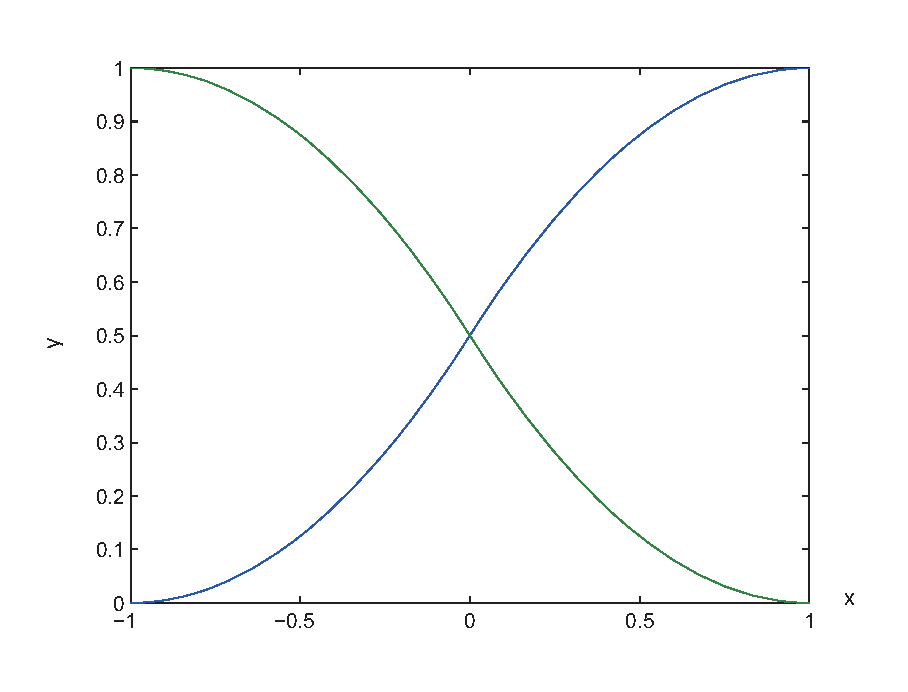
\includegraphics[width = 0.3\textwidth]{test1}
    \DeclareGraphicsExtensions.
  }
  \subfigure[$D=0.5$]{ \label{fig:ex1:resD:b}
    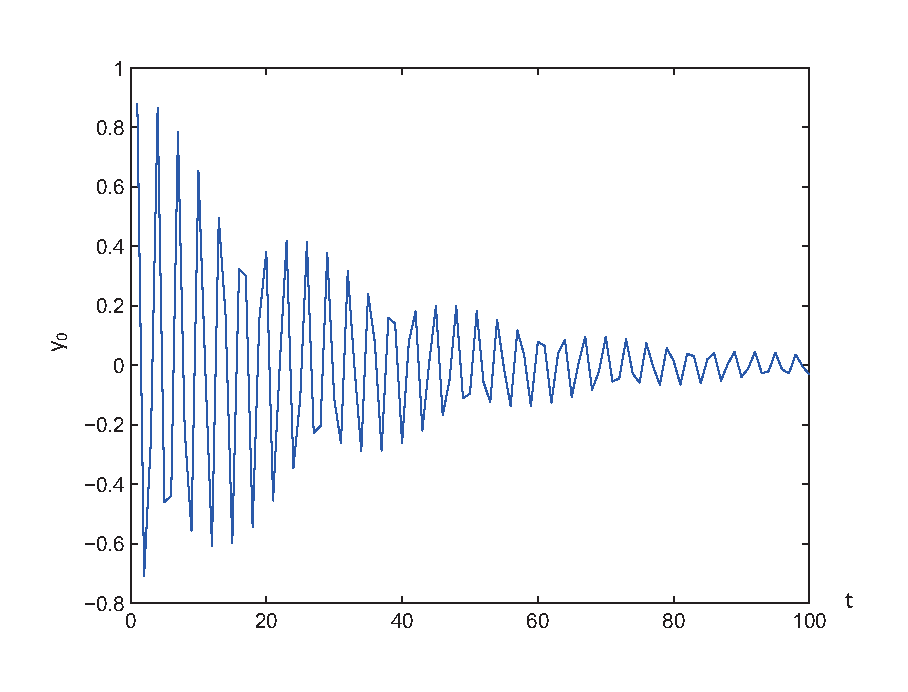
\includegraphics[width = 0.3\textwidth]{test2}
    \DeclareGraphicsExtensions.
  }
  \DeclareGraphicsExtensions.
  \caption{Test graphs.}\label{fig:ex1:resD}
\end{figure}
\end{frame}


%-------------------------------------------------------
\begin{frame}{Examples}{Equations}
%-------------------------------------------------------
\begin{itemize}
  \item Test blocked equations, i.e. \eqref{fml:eq1:partialW}, \eqref{fml:eq1:partialb}.
\end{itemize}

\begin{block}{SVM loss function} \label{blc:eq1}
  Here we show a simple example of subequations in \eqref{fml:eq1:partialW}:
  \begin{subequations}
    \renewcommand{\theequation}
    {\theparentequation-\arabic{equation}}
    \begin{align}
      \frac{\partial \mathcal{L}(\mathbf{w},~b)}{\partial \mathbf{w}} &= \mathbf{w} + C \sum\limits_i\frac{\partial \ell_i}{\partial \mathbf{w}}, \label{fml:eq1:partialW}\\
      \frac{\partial \mathcal{L}(\mathbf{w},~b)}{\partial b} &= C \sum\limits_i\frac{\partial \ell_i}{\partial b}, \label{fml:eq1:partialb}
    \end{align}
  \end{subequations}
\end{block}
\end{frame}


%-------------------------------------------------------
\begin{frame}{Examples}{Theorems}
%-------------------------------------------------------
\begin{itemize}
  \item Test theorems, i.e. \cref{thm:th1} and \cref{thm:th2}.
\end{itemize}

\begin{columns}
  \begin{column}{.48\textwidth}
    \begin{theorem}[Example Theorem 1] \label{thm:th1}
      Nam dui ligula, fringilla a, euismod
      sodales, sollicitudin vel, wisi. Morbi
      auctor lorem non justo. Nam lacus
      libero, pretium at, lobortis vitae,
      ultricies et, tellus. Donec aliquet,
      tortor sed accumsan bibendum, erat
      ligula aliquet magna, vitae ornare
      odio metus a mi.
    \end{theorem}
  \end{column}
  \begin{column}{.48\textwidth}
    \begin{theorem}[Example Theorem 2] \label{thm:th2}
      Quisque ullamcorper placerat ipsum.
      Cras nibh. Morbi vel justo vitae lacus
      tincidunt ultrices. Lorem ipsum dolor
      sit amet, consectetuer adipiscing elit.
      In hac habitasse platea dictumst.
      Integer tempus convallis augue.
      Etiam facilisis. Nunc elementum
      fermentum wisi.
    \end{theorem}
  \end{column}
\end{columns}
\end{frame}


%-------------------------------------------------------
\begin{frame}{Examples}{Algorithm}
%-------------------------------------------------------
\begin{itemize}
  \item Test algorithm, i.e. \cref{alg::Algorithm}.
\end{itemize}

\begin{algorithm}[H]
  \caption{DWT Algorithm}
  \label{alg::Algorithm}
  \begin{algorithmic}[1]
    \REQUIRE Sequence $\mathbf{x}$ in time domain
    \ENSURE Sequence $\hat{\mathbf{x}}$ in wavelet domain
    % if-then-else
    \STATE N = $\left\lfloor \log_2 (\mathrm{length}(\mathbf{x})) \right\rfloor$;
    \STATE $\mathbf{c}_{N} = \mathbf{x},~ \hat{\mathbf{x}} = \varnothing$;
    \FOR{$i$ from $1$ to $N$}
    \STATE $\mathbf{c}_{N-i},~\mathbf{d}_{N-i}~=~\mathrm{analysis\_filter}(\mathbf{c}_{N-i+1})$;
    \STATE insert $\mathbf{d}_{N-i}$ at the beginning of $\hat{\mathbf{x}}$.
    \ENDFOR
  \end{algorithmic}
\end{algorithm}
\end{frame}


\finalframe

\end{document}